\documentclass[pdflatex,sn-mathphys-num]{sn-jnl}

\usepackage{graphicx}
\usepackage{multirow}
\usepackage{amsmath,amssymb,amsfonts}
\usepackage{amsthm}
\usepackage{mathrsfs}
\usepackage[title]{appendix}
\usepackage{xcolor}
\usepackage{colortbl}
\usepackage{textcomp}
\usepackage{manyfoot}
\usepackage{booktabs}
\usepackage{tikz}
\usetikzlibrary{shapes,arrows,positioning,calc,fit,backgrounds}
\usepackage{subcaption}
\usepackage{fontawesome5}
\usepackage{xspace}
\usepackage[nohyperlinks]{acronym}
\acrodef{A2V}{Audio-to-Video}
\acrodef{AQ}{Aesthetic Quality}
\acrodef{AU}{Action Unit}
\acrodef{VFX}{Visual Effects}
\acrodef{DiT}{Diffusion Transformer}
\acrodef{EI}{Emotional Intensity}
\acrodef{ER}{Expression Realism}
\acrodef{FACS}{Facial Action Coding System}
\acrodef{GAN}{Generative Adversarial Network}
\acrodef{GenAI}{Generative Artificial Intelligence}
\acrodef{LDM}{Latent Diffusion Model}
\acrodef{MoCap}{Motion Picture Capture}
\acrodef{ODE}{Ordinary Differential Equation}
\acrodef{T2V}{Text-to-Video}
\acrodef{TC}{Temporal Coherence}

\newcommand{\emAnger}{Anger\xspace}
\newcommand{\emEncouragement}{Encouragement\xspace}
\newcommand{\emJoy}{Joy\xspace}
\newcommand{\emGratitude}{Gratitude\xspace}
\newcommand{\Pone}{\colorbox{gray!15}{P1}\xspace}
\newcommand{\Ptwo}{\colorbox{gray!30}{P2}\xspace}

\definecolor{cadmiumgreen}{rgb}{0.0, 0.42, 0.24}
\newcommand{\gray}[1]{{\color{gray}#1}}
\newcommand{\blue}[1]{{\color{blue}#1}}
\newcommand{\cadmiumgreen}[1]{{\color{cadmiumgreen}#1}}
\newcommand{\foo}{\hspace{1em}}


\theoremstyle{thmstyleone}
\newtheorem{theorem}{Theorem}
\newtheorem{proposition}[theorem]{Proposition}%
\theoremstyle{thmstyletwo}
\newtheorem{example}{Example}
\newtheorem{remark}{Remark}
\theoremstyle{thmstylethree}
\newtheorem{definition}{Definition}
\raggedbottom


\begin{document}

\title[]{AI-Generated Human Avatars: Emotion Fidelity Evaluation and Societal Impacts}

\author*[1]{\fnm{Alan} \sur{Guedes}}\email{a.guedes@reading.ac.uk}
\author[2]{\fnm{Dominic} \sur{Lees}}\email{d.lees@reading.ac.uk}
\affil*[1]{\orgdiv{Department of Computer Science}, \orgname{University of Reading}, \orgaddress{\city{Reading}, \country{United Kingdom}}}
\affil[2]{\orgdiv{Department of Film, Theatre \& Television}, \orgname{University of Reading}, \orgaddress{\city{Reading}, \country{United Kingdom}}}

\abstract{ This paper presents a multi-disciplinary evaluation of emotional fidelity of Humans Avatar in videos generated by state-of-the-art \ac{GenAI} models. Through a structured focus group session with film industry researchers, we assess the performance of HunyuanVideo-Avatar and Runway across text-to-video and audio-driven generation tasks. While current generative architectures achieve high visual quality, we identify significant limitations in their capacity to express subtle, complex human emotions. We examine these constraints, mapping the evolution of recent models and detailing the specific emotional expression deficits observed. We contextualize these results within the broader discussion of the responsible use of AI in art creation and archival practice, proposing frameworks that prioritize human artistic agency.}

\keywords{Generative AI, Humans Avatars, Video Synthesis}

\maketitle
\acresetall

\section{Introduction}\label{sec1}
The rapid advancement of \ac{GenAI} has introduced a paradigm shift in visual media production and character synthesis. Historically, digital human avatars have achieved remarkable visual and emotional fidelity when driven by traditional \ac{VFX} workflows and \ac{MoCap} systems, which track physical actor performances to animate underlying blendshape rigs. Today, a powerful new paradigm has emerged: complete autonomous video generation, where photorealistic digital avatars are synthesized dynamically from text prompts via \ac{T2V} and speech audio via \ac{A2V} pipelines, operating entirely without motion capture suits, tracking markers, or physical performer guidance.


\begin{table*}[ht!]
\centering
\caption{Overview of digital human avatar synthesis paradigms.}
\label{tab:paradigm_evolution}
\makebox[\textwidth][c]{%
\begin{tabular}{cc}
\toprule
\multicolumn{2}{c}{\textbf{\large Human Avatar from MoCap and \ac{VFX}}\footnotemark\textsuperscript{,}\footnotemark} \\
\midrule
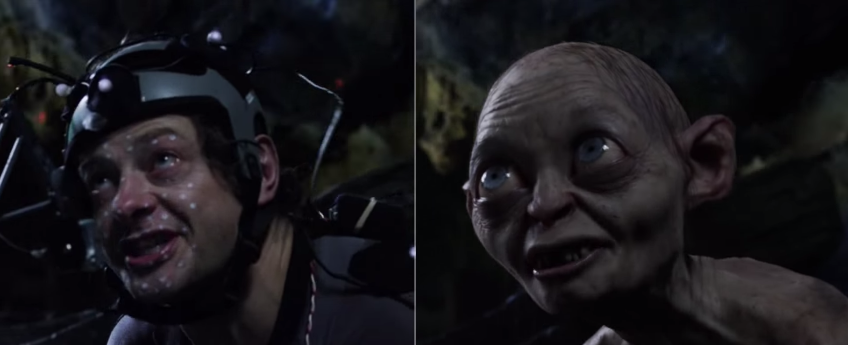
\includegraphics[width=0.48\textwidth,height=3.0cm]{assets/gollum.png} &
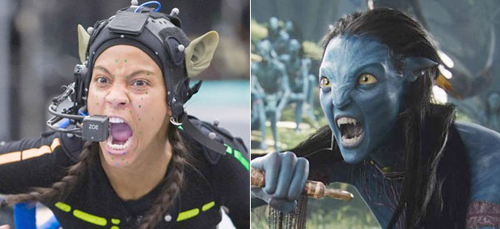
\includegraphics[width=0.48\textwidth,height=3.0cm]{assets/avatar.png} \\
\midrule
\multicolumn{2}{c}{\textbf{\large Human Avatar from MoCap and GenAI}\footnotemark\textsuperscript{,}\footnotemark} \\
\midrule
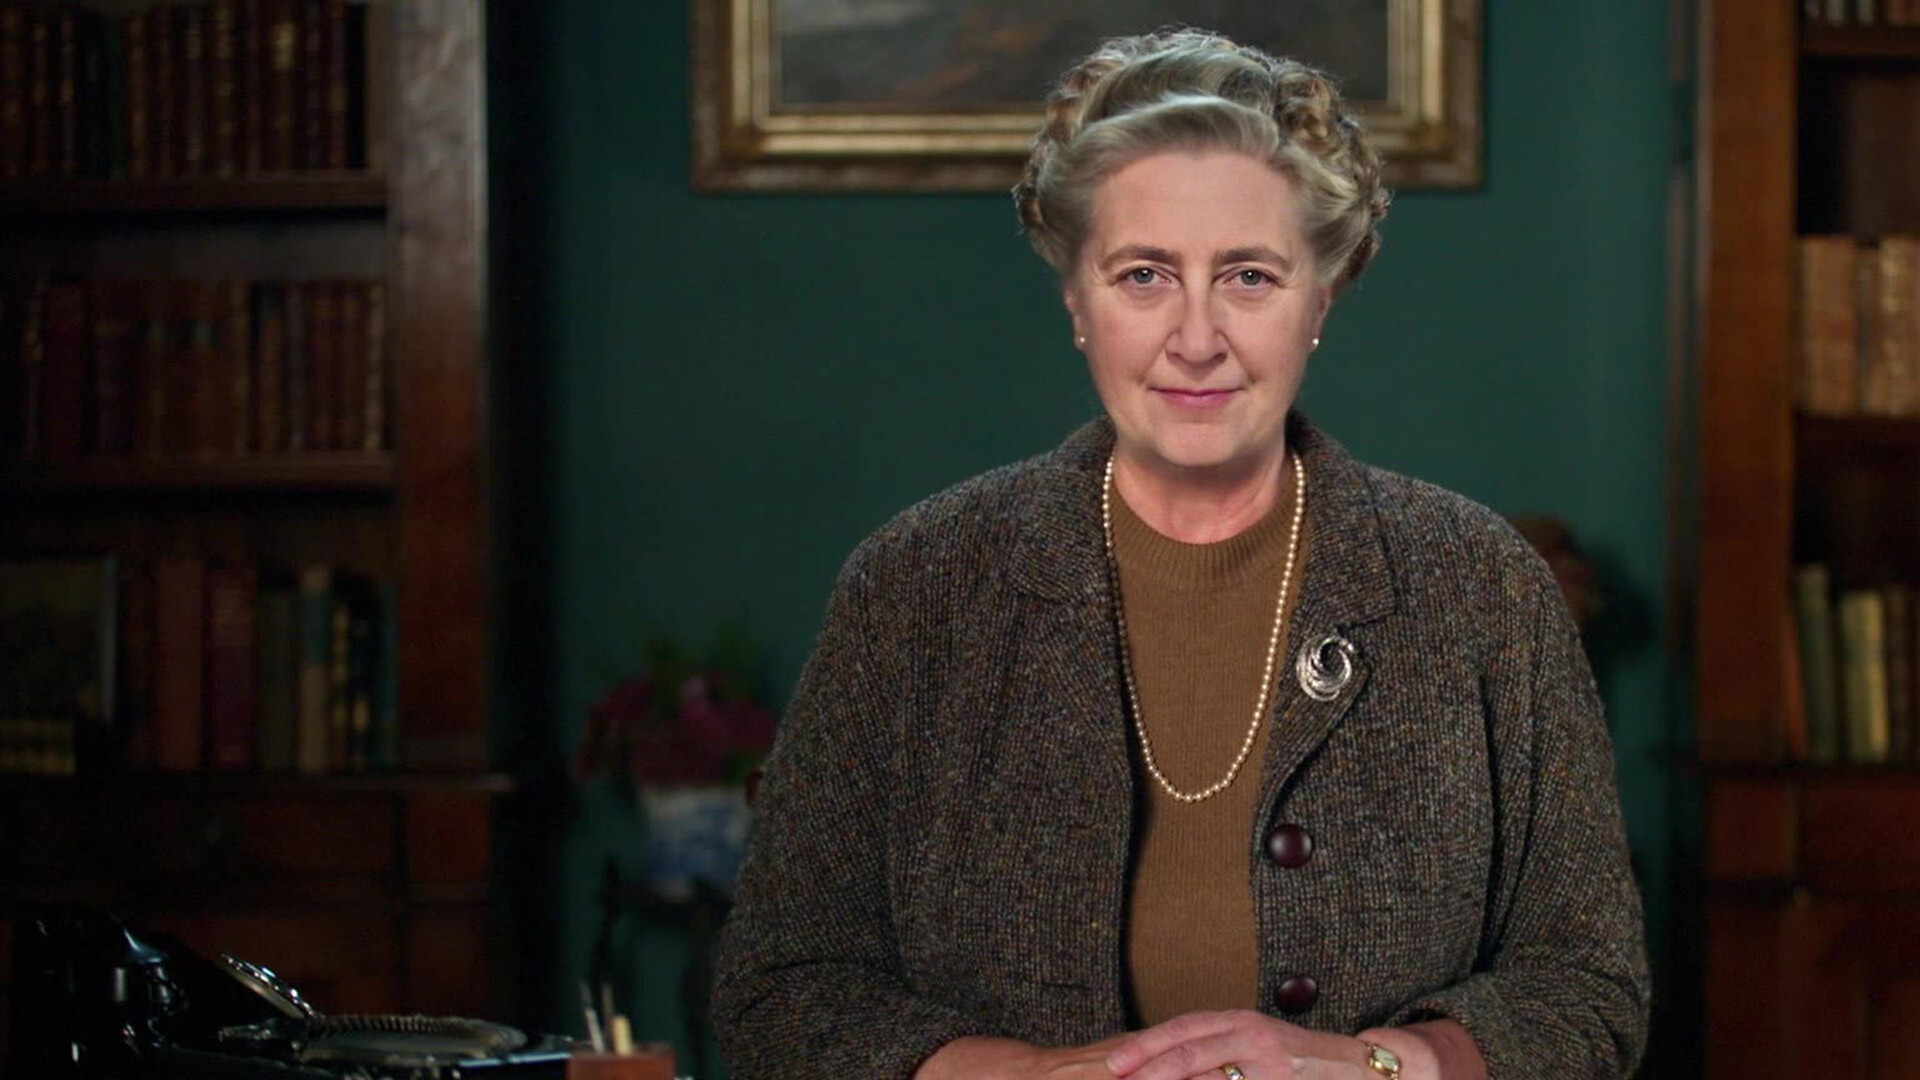
\includegraphics[width=0.48\textwidth,height=3.0cm]{assets/agatha.png} &
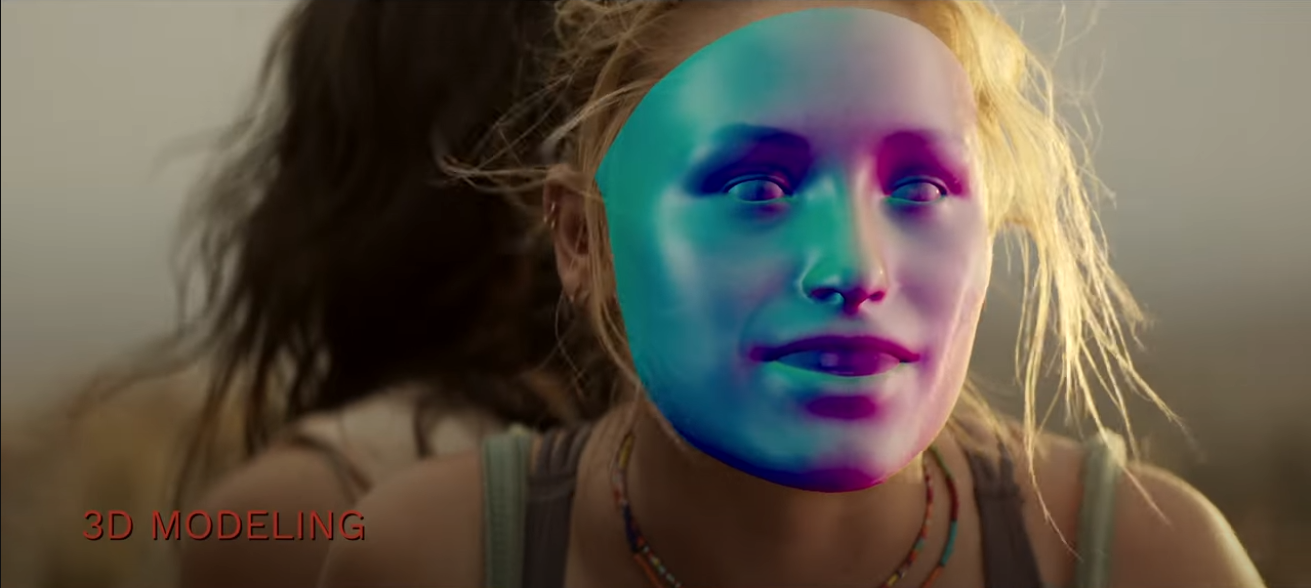
\includegraphics[width=0.48\textwidth,height=3.0cm]{assets/replace1.png} \\
\midrule
\multicolumn{2}{c}{\textbf{\large Human Avatar from GenAI}\footnotemark} \\
\midrule
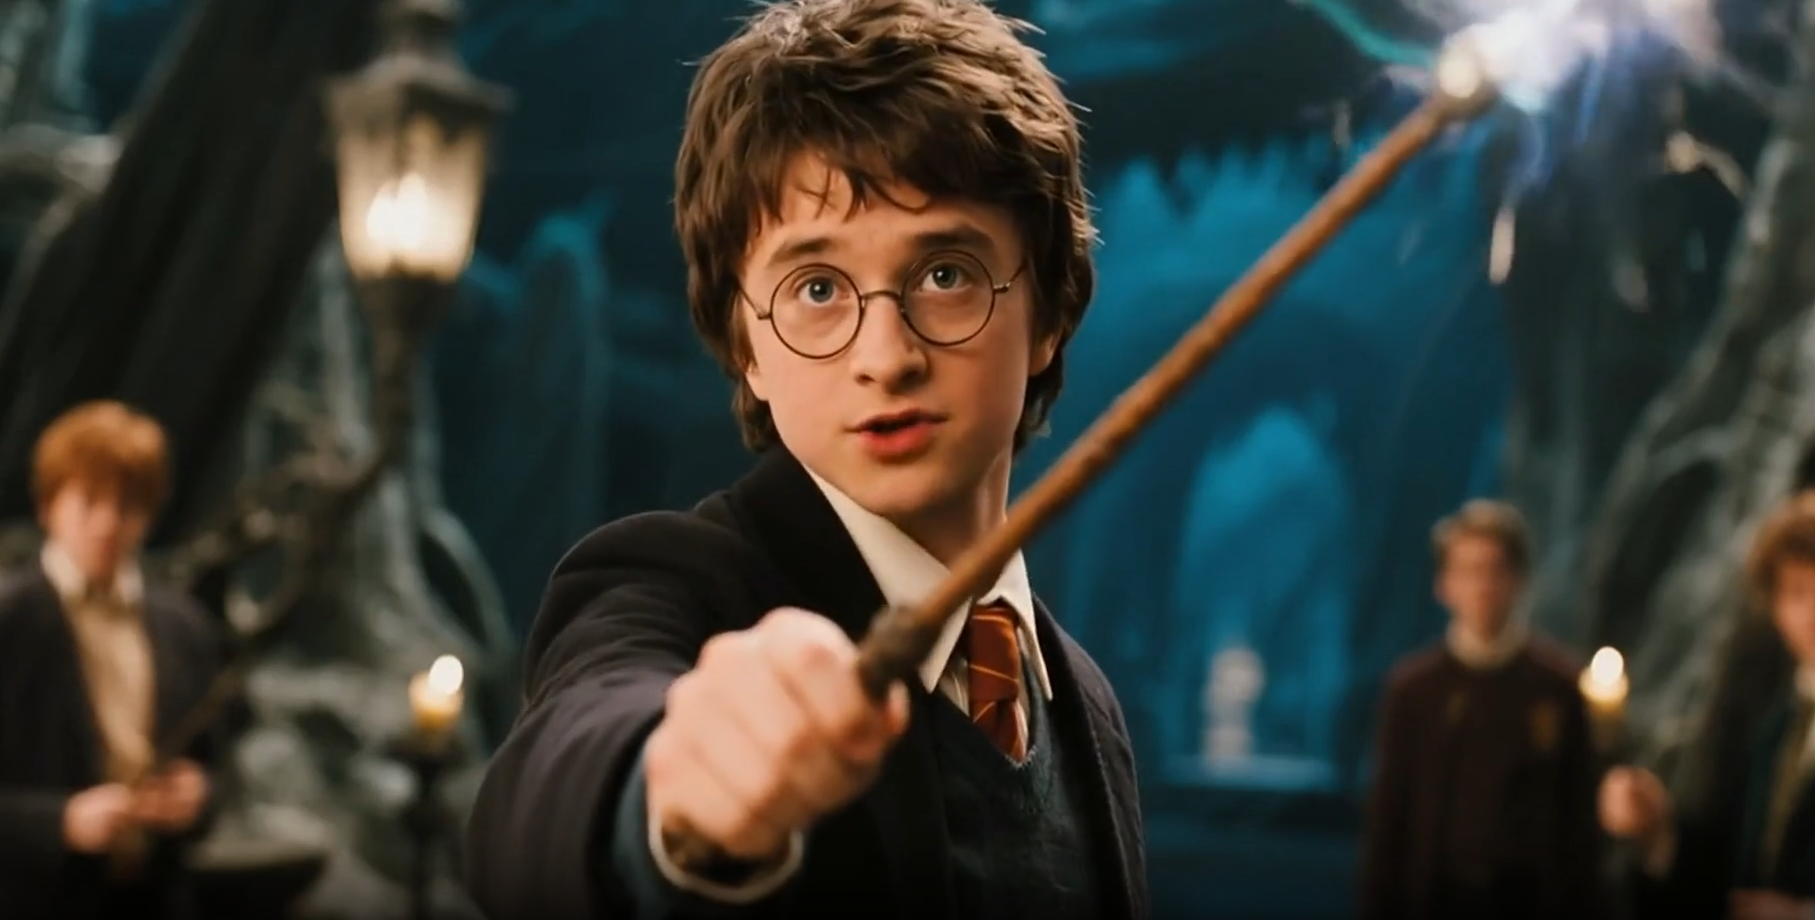
\includegraphics[width=0.48\textwidth,height=3.0cm]{assets/hunyuanvideo-avatar.png} &
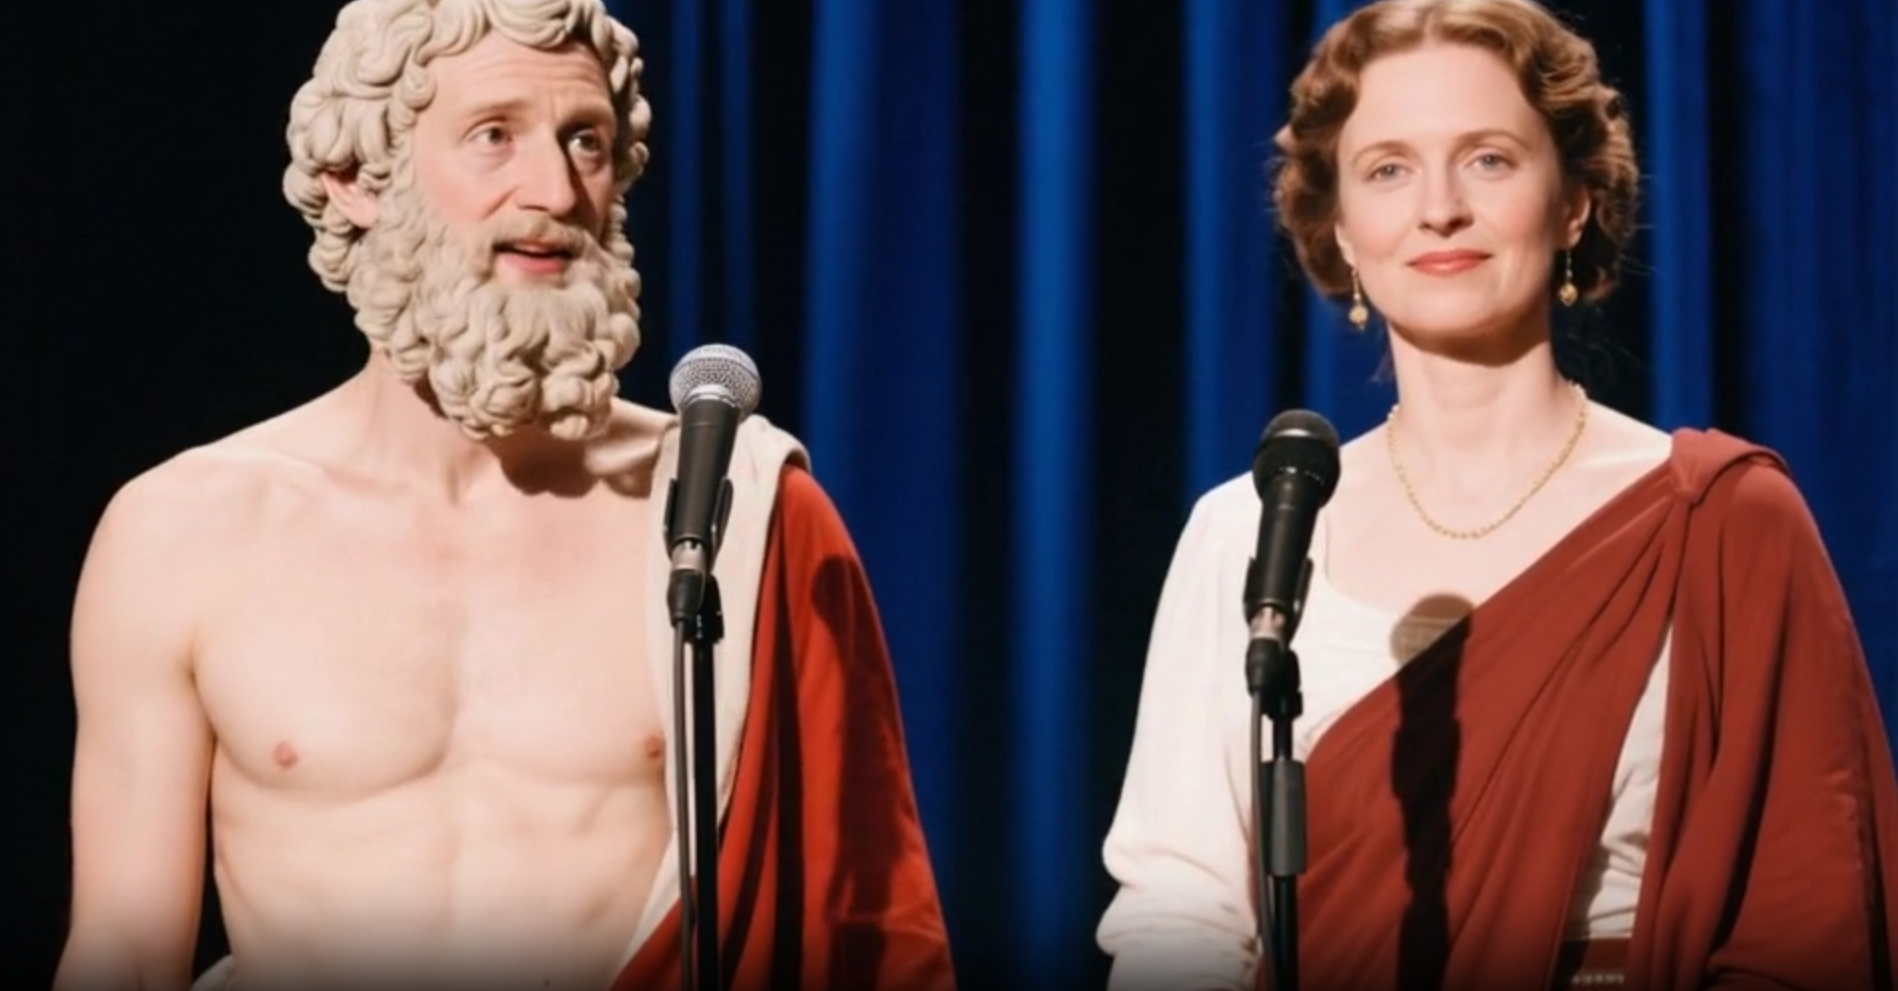
\includegraphics[width=0.48\textwidth,height=3.0cm]{assets/hunyuanvideo-avatar2.png} \\
\bottomrule
\end{tabular}%
}
\end{table*}
\footnotetext{\url{https://themagicpuppetvfx.wordpress.com/2014/06/06/motion-capture-and-creation-of-the-apes-weta-digital/}}
\footnotetext{\url{https://beforesandafters.com/2022/09/19/watch-this-official-avatar-perfoarmance-capture-featurette/}}
\footnotetext{\url{https://www.bbcmaestro.com/courses/agatha-christie/writing}}
\footnotetext{\url{https://www.flawlessai.com/}}
\footnotetext{\url{https://hunyuanvideo-avatar.com/}}


This transition from performer-driven \ac{MoCap} to unconstrained, autonomous generation raises two fundamental questions. First, \textit{how good are these autonomous \ac{T2V} and \ac{A2V} avatars at conveying nuanced emotional performance?} Deprived of physical anatomical tracking and biomechanical rig constraints, latent diffusion models synthesize animation purely through statistical correlations, frequently causing emotional flattening, Duchenne smile deficits, and spatial warping under high emotional intensity. Second, \textit{how good are open-source, auditable models compared to commercial proprietary systems?} While commercial black-box models deliver high visual surface polish, they conceal their training data distributions, safety alignment procedures, and internal mechanics. Evaluating open-source, inspectable architectures (such as HunyuanVideo-Avatar~\cite{hunyuan2025avatar}) is critical to determine whether accessible, ethically auditable models can achieve competitive expressive fidelity while enabling researchers to examine their underlying cross-modal internal representations (i.e., latent spaces).

This raises two central research questions: 
\begin{itemize}
    \item \textbf{RQ1:} \textit{how the humans avatar models handle emotion fidelity?}
    \item \textbf{RQ2:} \textit{How open-source and auditable models are compared to proprietary ones?}
\end{itemize}

Through a structured focus group session conducted with Film and Television academic and student researchers at [Anonymized University], we perform a qualitative evaluation of state-of-the-art open-source and commercial video generation models (HunyuanVideo-Avatar and Runway) across text-to-video (T2V) and audio-driven video synthesis pipelines. Identifying structural limitations such as Duchenne smile deficits, physical warping, and cross-modal disconnections, we argue for a more responsible, human-centric design of generative tools that respects acting heritage and supports rather than replaces creative human agency. To this end, a primary contribution of this work is establishing an evaluation paradigm that addresses both \textbf{Quality Dimensions} (Aesthetic Quality, Expression Realism, Emotional Intensity, and Temporal Coherence) and \textbf{Ethical Dimensions} (model auditability, training data provenance, performer consent, labor rights, and digital likeness governance, building on policy research by Pavis and Lees~\cite{pavis2025ai, signapselinkedin}). Specifically, our contributions are threefold: first, a multi-disciplinary qualitative evaluation of state-of-the-art GenAI models in text-to-video and audio-driven contexts; second, a framework structured around core Quality Dimensions to assess performance depth; and third, an analysis of Ethical Dimensions examining contract patterns, labor protections, and contrasting international regulatory frameworks (including the EU AI Act and US copyright rulings) for synthetic likeness governance.

The remainder of this paper is structured as follows. Section~\ref{sec:mocap_systems} provides the background on digital avatar synthesis and the transition to generative networks. Section~\ref{sec3} details our evaluation methodology, results, and discussion. Section~\ref{sec5:societal} addresses the societal, policy, and legal dimensions of digital likeness, contrasting international regulatory regimes. Finally, Section~\ref{sec6} concludes the paper.


\section{Background}\label{sec:mocap_systems}

\begin{table}[ht!]
\caption{Historical timeline humans avatar generation methods.}\label{tab:evolution_timeline}
\begin{tabular}{l | @{\foo} p{10.5cm}}
    1978 & Ekman and Friesen publish the Facial Action Coding System (FACS)~\cite{ekman1978facial} \\
    1990s--2010s & Optical motion capture (MoCap) rigs and performance capture become movie industry standards \\
    2014 & Goodfellow et al. propose Generative Adversarial Networks (GANs)~\cite{goodfellow2014generative} \\
    2019 & Karras et al. introduce StyleGAN for high-fidelity static face synthesis~\cite{karras2019style} \\
    2020--2022 & Early video GANs (e.g., MoCoGAN) attempt video synthesis, but with low resolution  \\
    2022 & Rombach et al. introduce Latent Diffusion Models (LDMs)~\cite{rombach2022high} \\
    2023 & Stable Video Diffusion and Runway Gen-2 scale video generation, suffer from prompt drift and warping \\
    2023 & Peebles and Xie propose Diffusion Transformers (DiTs)~\cite{peebles2023scalable} \\
    2024 & Lipman et al. introduce Flow Matching for straight-path modeling~\cite{lipman2022flow} \\
         & Runway Gen-3 Alpha and HunyuanVideo-Avatar integrate DiTs for highly stable character generation~\cite{hunyuan2025avatar,runway2024gen3} \\
    2025 & HunyuanVideo-Avatar open-source audio-driven video model released~\cite{hunyuan2025avatar} \\
\end{tabular}
\end{table}

The historical timeline in Table~\ref{tab:evolution_timeline} charts the transition from anatomical classification systems and physical motion capture (MoCap) to data-driven statistical models for character synthesis. Grounded in the Facial Action Coding System (FACS)~\cite{ekman1978facial}, classic production pipelines relied on optical MoCap rigs, head-mounted camera (HMC) arrays, and performance capture to track physical actor kinesics. Milestone cinematic productions demonstrated the expressive fidelity of these physical capture pipelines (Table~\ref{tab:paradigm_evolution}), from Weta Digital's body motion capture of Gollum in \textit{The Lord of the Rings} to HMC facial tracking in James Cameron's \textit{Avatar}. While physical MoCap guarantees temporal consistency and precise artistic control, it remains labor-intensive and costly. The following subsections examine the shift toward statistical learning, detailing human avatars driven by MoCap and GenAI (Section~\ref{sec:face_gen_mocap}) and human avatars synthesized purely via GenAI (Section~\ref{sec:human_video_gen}).

\subsection{Human Avatar from MoCap and GenAI}\label{sec:face_gen_mocap}
The transition from physical performance to digital character synthesis has occurred in distinct waves, moving from rigid geometric control to dynamic statistical estimation. Prominent examples of these technologies, such as the viral Tom Cruise TikTok deepfakes\footnote{\url{https://www.cnet.com/culture/internet/creator-of-tom-cruise-deepfakes-shares-how-he-made-those-viral-tiktok-videos/}} and the Jordan Peele/BuzzFeed Obama deepfake address\footnote{\url{https://ars.electronica.art/center/en/obama-deep-fake/}}, brought the capability and societal impact of synthetic avatars into public awareness.

\textbf{Early GAN and LDM Frameworks.} Early approaches utilized Generative Adversarial Networks (GANs)~\cite{goodfellow2014generative}, such as StyleGAN~\cite{karras2019style}, to generate high-fidelity static faces. Extending them to video required architectures like VideoGAN or MoCoGAN, which split internal representations (i.e., latent spaces) into spatial content and motion vectors. These early video GANs suffered from low resolution, "mode collapse," and massive temporal drift. The subsequent introduction of Latent Diffusion Models (LDMs)~\cite{rombach2022high} solved many resolution challenges by executing the diffusion process in a compressed, low-dimensional internal representation (i.e., latent space), enabling applications like the BBC Agatha Christie content generation course~\cite{bbcmaestroagatha} (Table~\ref{tab:paradigm_evolution}). However, early models like Runway Gen-2 still exhibited significant prompt drift, physical clipping under movement, and a lack of three-dimensional structural consistency, hindering their application in precise film dialogue replacement~\cite{truesyncdialogue} (Table~\ref{tab:paradigm_evolution}).

\subsection{Human Avatar from GenAI}\label{sec:human_video_gen}

Modern video generation has transitioned to data-driven statistical scaling, shifting the spatial backbone of video models from U-Nets to Diffusion Transformers (DiTs)~\cite{peebles2023scalable}. The video latent volume is partitioned into non-overlapping 3D spatial-temporal patches, projected as token sequences, and combined with 3D positional encodings (e.g., RoPE) to capture global spatial and temporal dependencies through self-attention layers. Conditioning inputs, such as text prompts (via T5) or speech audio (via Wav2Vec~\cite{baevski2020wav2vec}), are injected via cross-attention. Recent audio-driven avatar frameworks like EMO~\cite{tian2024emo}, DiceTalk~\cite{dicetalk2025}, and RETA~\cite{reta2026}, alongside emotion-conditioned generation models such as Emotion-Director~\cite{emotiondirector2025} and EmotiCrafter~\cite{emoticrafter2025}, attempt to improve expressive control.

To optimize the generation process, these pipelines implement Flow Matching~\cite{lipman2022flow}, which defines a deterministic vector field to generate straight-path trajectories in the internal representation (i.e., latent space), allowing standard numerical \ac{ODE} solvers to synthesize stable videos in only 20--30 steps. Although this transformer-based latent mapping scales effectively in open-source models like Hunyuan-Video~\cite{hunyuan2024video} and HunyuanVideo-Avatar\footnote{\url{https://hunyuanvideo-avatar.com/}}~\cite{hunyuan2025avatar} (demonstrated in Table~\ref{tab:paradigm_evolution}) and Runway Gen-3 Alpha~\cite{runway2024gen3}, it remains a statistical estimator. Lacking biophysical, skeletal, or anatomical constraints, it relies purely on statistical correlations, resulting in the emotional and physical performance distortions observed in our evaluations.

\begin{figure}[ht!]
  \centering
  \resizebox{\textwidth}{!}{%
  \begin{tikzpicture}[
    node distance=1.2cm and 1.5cm,
    block/.style={draw, fill=gray!15, rectangle, minimum height=2.2em, minimum width=7.5em, rounded corners, align=center, font=\small},
    input/.style={draw, fill=white, rectangle, minimum height=2.2em, minimum width=7em, align=center, font=\small},
    process/.style={draw, fill=gray!30, rectangle, minimum height=2.2em, minimum width=8.5em, rounded corners, align=center, font=\small},
    arrow/.style={draw, ->, >=stealth, thick}
  ]
    \node [input] (text) {\faKeyboard~Text Prompt};
    \node [input, below=0.8cm of text] (audio) {\faMusic~Audio Input};
    
    \node [block, right=of text] (text_enc) {Text Encoder\\(e.g., T5)};
    \node [block, right=of audio] (audio_enc) {Audio Encoder\\(e.g., Wav2Vec)};
    
    \node [process, right=1.2cm of $(text_enc.east)!0.5!(audio_enc.east)$] (conditioning) {Cross-Attention \&\\Conditioning Layer};
    
    \node [block, right=1.2cm of conditioning] (dit) {Diffusion Transformer\\(DiT) Blocks};
    
    \node [input, right=of dit] (output) {\faVideo~Generated\\Video Output};
    
    \draw [arrow] (text) -- (text_enc);
    \draw [arrow] (audio) -- (audio_enc);
    \draw [arrow] (text_enc.east) -- ++(0.4,0) |- (conditioning.west);
    \draw [arrow] (audio_enc.east) -- ++(0.4,0) |- (conditioning.west);
    \draw [arrow] (conditioning) -- (dit);
    \draw [arrow] (dit) -- (output);
    
  \end{tikzpicture}
  }
  \caption{Conditioning pathways in modern Diffusion Transformer (DiT) video generation architectures, supporting both text-only generation (top pipeline) and audio-guided generation (bottom pipeline) conditioning noisy video patches.}
  \label{fig:dit_architecture}
\end{figure}

\section{Qualitative Evaluation of Emotion Fidelity}\label{sec3}

\begin{figure}[ht!]
  \centering
  \resizebox{\textwidth}{!}{
  \begin{tikzpicture}[
    node distance=1.5cm,
    block/.style={draw=black!70, fill=gray!10, rectangle, rounded corners, thick, align=center, inner sep=10pt, font=\small, minimum width=4cm, minimum height=1.5cm},
    input/.style={draw=black!40, fill=gray!2, dashed, rectangle, rounded corners, align=center, inner sep=6pt, font=\footnotesize, minimum width=3.5cm},
    arrow/.style={draw, ->, >=stealth, thick, black!70}
  ]
    \node [input] (audio) {\faMusic~\textbf{Audio Input}\\(e.g., J. Nicholson voice)};
    \node [input, below=0.4cm of audio] (ref) {\faImage~\textbf{Reference Image}\\(e.g., J. Nicholson frame)};
    
    \node [block, right=1.2cm of audio, yshift=-0.5cm] (gen) {\faVideo~\textbf{Video Generation}\\(HunyuanVideo-Avatar / Runway Gen-3)};
    \node [block, right=of gen] (analysis) {\faUser\quad\faClipboardCheck~\textbf{FTT Analysis}\\(P1/P2 Evaluation)};
    \node [block, right=of analysis] (summary) {\faComments~\textbf{Feedback Summary}\\(Quality Dimensions)};
    
    \draw [arrow] (audio.east) -- ++(0.4,0) |- ([yshift=0.2cm]gen.west);
    \draw [arrow] (ref.east) -- ++(0.4,0) |- ([yshift=-0.2cm]gen.west);
    \draw [arrow] (gen) -- (analysis);
    \draw [arrow] (analysis) -- (summary);
  \end{tikzpicture}
  }
  \caption{Evaluation workflow framework.}
  \label{fig:audio_generation_pipeline}
\end{figure}To evaluate how state-of-the-art generative models capture human emotion, we designed a structured focus group evaluation. This evaluation tracks the fidelity of synthetic avatars created from iconic movie scenes across different generation pipelines. We analyze the process of exporting generated video frames and managing key frames to assess motion consistency and temporal degradation. To address both RQ1 (emotional acting replication) and RQ2 (open-source vs. proprietary architectures), we designed our evaluation to directly contrast commercial, proprietary foundation models (Model A: Runway Gen-3 Alpha) against open-source, auditable architectures (Model B: HunyuanVideo-Avatar). While foundational open-source text-to-video Diffusion Transformers such as Wan2.1 and Hunyuan-Video establish state-of-the-art visual generation capabilities, they operate without direct audio speech driving; thus, they provide valuable architectural background but were not part of our empirical focus group trials. While proprietary models offer high visual resolution, their closed nature prevents auditing the training data or underlying alignment. Open-source models, on the other hand, permit inspecting their weights and intermediate latent layers, which is crucial for auditing representations of diverse physical features and expressions. In the following subsections, we discuss the video generation process and the qualitative evaluation from industry experts.

\subsection{Video Generation}\label{subsec:video_generation}

To evaluate the current state of emotional performance in generative video, this study focuses on audio-driven facial synthesis, which represents a sub-field of video generation where speech audio animates a digital character. Early models like Wav2Lip utilized discriminators to enforce lip-sync accuracy, while models like SadTalker introduced facial landmark generators to simulate natural head motion and blinking. In contemporary pipelines, such as HunyuanVideo-Avatar, speech audio is processed through audio encoders (like Wav2Vec) and mapped directly to spatial-temporal internal representations (i.e., latent spaces). While these models achieve highly accurate lip-syncing, they suffer from a severe "emotional disconnect." Because they map phonemes to lip movements, they fail to model the emotional state of the speaker. A trembling, tearful voice track will animate the lips to form the correct words, but the eyes, forehead, and cheeks will remain static and unexpressive.

All video generation and evaluation trials were executed using the ComfyUI platform\footnote{\url{https://alanlivio.github.io/paper-eval-genai-movie-characters/}} on identical workstations equipped with AMD Ryzen 9 5900X processors, 64 GB of DDR4 RAM, and NVIDIA GeForce RTX 4090 GPUs (24 GB VRAM).

To empirically evaluate the emotional limitations of these architectures, we conducted a qualitative evaluation of audio-driven performance synthesis using four iconic scenes from classic cinema. These scenes were selected to cover a wide spectrum of emotional intensity and expressive complexity:

\begin{itemize}
    \item \textbf{\emAnger:} Jack Nicholson's courtroom monologue in \textit{A Few Good Men} (\url{https://www.youtube.com/watch?v=2sLcfQKU_co}). This scene was selected to evaluate explosive vocal projection, clenched jaw muscles, dynamic head movements, and facial micro-expressions of contempt under high-intensity rage.
    \item \textbf{\emEncouragement:} Sylvester Stallone's inspirational speech to his son in \textit{Rocky Balboa} (\url{https://www.youtube.com/watch?v=D_Vg4uyYwEk}). This scene was selected to evaluate the model's ability to sync speech audio under lower vocal frequencies while maintaining consistent jaw articulation and concentrated, emotionally charged eye contact.
    \item \textbf{\emJoy:} Robin Williams' class scenes in \textit{Dead Poets Society} (\url{https://www.youtube.com/watch?v=Wey8nauEyA4}). This scene was selected to evaluate how models capture warm, natural transitions of genuine joy, facial animation during smiles, and relaxed eye involvement.
    \item \textbf{\emGratitude:} Robin Williams and Matt Damon's counseling scene ("It's not your fault") in \textit{Good Will Hunting} (\url{https://www.youtube.com/watch?v=8SxE_NfUX6w}). This scene was selected to evaluate the expression of vulnerability, subtle eye movements, vocal trembling, and the complex emotional delivery of gratitude and cathartic relief.
\end{itemize}

Character screenshots and the original actor voice tracks were extracted from these scenes and processed through Model A (Runway Gen-3 Alpha) and Model B (HunyuanVideo-Avatar) to generate corresponding synthetic characters.

\subsection{Evaluation Results}\label{subsec:qualitative_evaluation}

A focus group consisting of an academic researcher and an MSc student in Film and Television qualitatively compared the generated characters directly to the baseline actor performances, focusing on visual aesthetics, expression realism, emotional intensity, and temporal stability. To analyze the qualitative nuances across each evaluated emotion, we examine the feedback, observations, and rating scores (on a 1--10 scale) compiled in the expert columns of Table~\ref{tab:expert_feedback_anger_enc} and Table~\ref{tab:expert_feedback_joy_grat}, with detailed video outputs and comparative demos hosted on the companion project webpage\footnote{\url{https://magenta-crepe-43d98a.netlify.app}}:
\begin{itemize}
    \item \textbf{\emAnger:} In the Jack Nicholson courtroom monologue sequence, \Pone (Rating: 5/10) noted a stark contrast between Runway's high visual resolution and its flat, vacant expression delivery (the "blank stare"), observing that the eyes did not narrow and the brow remained un-furrowed despite the aggressive prompt. \Ptwo (Rating: 6/10) agreed that Runway's anger felt superficial, resembling a neutral mask with an open mouth. For HunyuanVideo-Avatar (\Pone: 2/10, \Ptwo: 1/10), both experts highlighted severe face warping and distortion, with \Pone observing that the teeth appeared to float independently, and \Ptwo noting that the animation broke the suspension of disbelief due to temporal inconsistencies and a jittery, disjointed head motion.
    \item \textbf{\emEncouragement:} For the Sylvester Stallone motivational speech, \Pone (Rating: 5/10) observed that Runway maintained a steady head pose but the eyes remained dead and unresponsive, with the lips moving but the rest of the face failing to participate. \Ptwo (Rating: 6/10) characterized this delivery as flat and robotic, pointing out the disconnect where the tone of voice suggests passion but the face suggests indifference. For HunyuanVideo-Avatar (\Pone: 4/10, \Ptwo: 1/10), \Pone noted the accurate lip-syncing but highlighted a failure to connect vocal intensity with upper facial expressions, while \Ptwo pointed out cheek distortions and sliding skin textures.
    \item \textbf{\emJoy:} In the Robin Williams classroom scene, \Pone (Rating: 5/10) noted that Runway's smile felt fake or "plastic," failing to engage the eyes (Duchenne smile deficit). \Ptwo (Rating: 2/10) characterized Runway's output as an animated stock photo lacking warm, natural transitions. For HunyuanVideo-Avatar (\Pone: 4/10, \Ptwo: 7/10), \Pone observed that the model struggled to keep facial structure stable while smiling, leading to melting or warping around the nose and mouth, while \Ptwo noted poor temporal coherence with teeth merging into a solid block despite appreciating its subtle facial rendering.
    \item \textbf{\emGratitude:} For the counseling scene, the cross-modal mismatch was highly pronounced. \Pone (Rating: 3/10) observed that Runway's emotional tone was lost, resulting in a blank look rather than appreciation, while \Ptwo (Rating: 6/10) noted that the character lacked micro-expressions of vulnerability, failing to project any internal psychological state. In the HunyuanVideo-Avatar version (\Pone: 4/10, \Ptwo: 1/10), \Pone observed that while the vocal track was trembling and emotional, the eyes remained vacant, and \Ptwo confirmed that the eye area remained static while the mouth shape changes.
\end{itemize}

\begin{table*}[ht]
\centering
\caption{Expert Feedback on \emAnger and \emEncouragement Expressions}
\label{tab:expert_feedback_anger_enc}
\makebox[\textwidth][c]{%
\begin{tabular}{p{2.8cm}p{2.8cm}>{\columncolor{gray!10}}p{5.0cm}>{\columncolor{gray!20}}p{5.0cm}}
\toprule
\textbf{Input} & \textbf{Output} & \textbf{P1} & \textbf{P2} \\
\midrule
{\centering
\raisebox{-.5\height}{
\includegraphics[width=2.5cm]{assets/actor_anger.png}} \par Anger scene \par\vspace{0.3cm}
\raisebox{-.5\height}{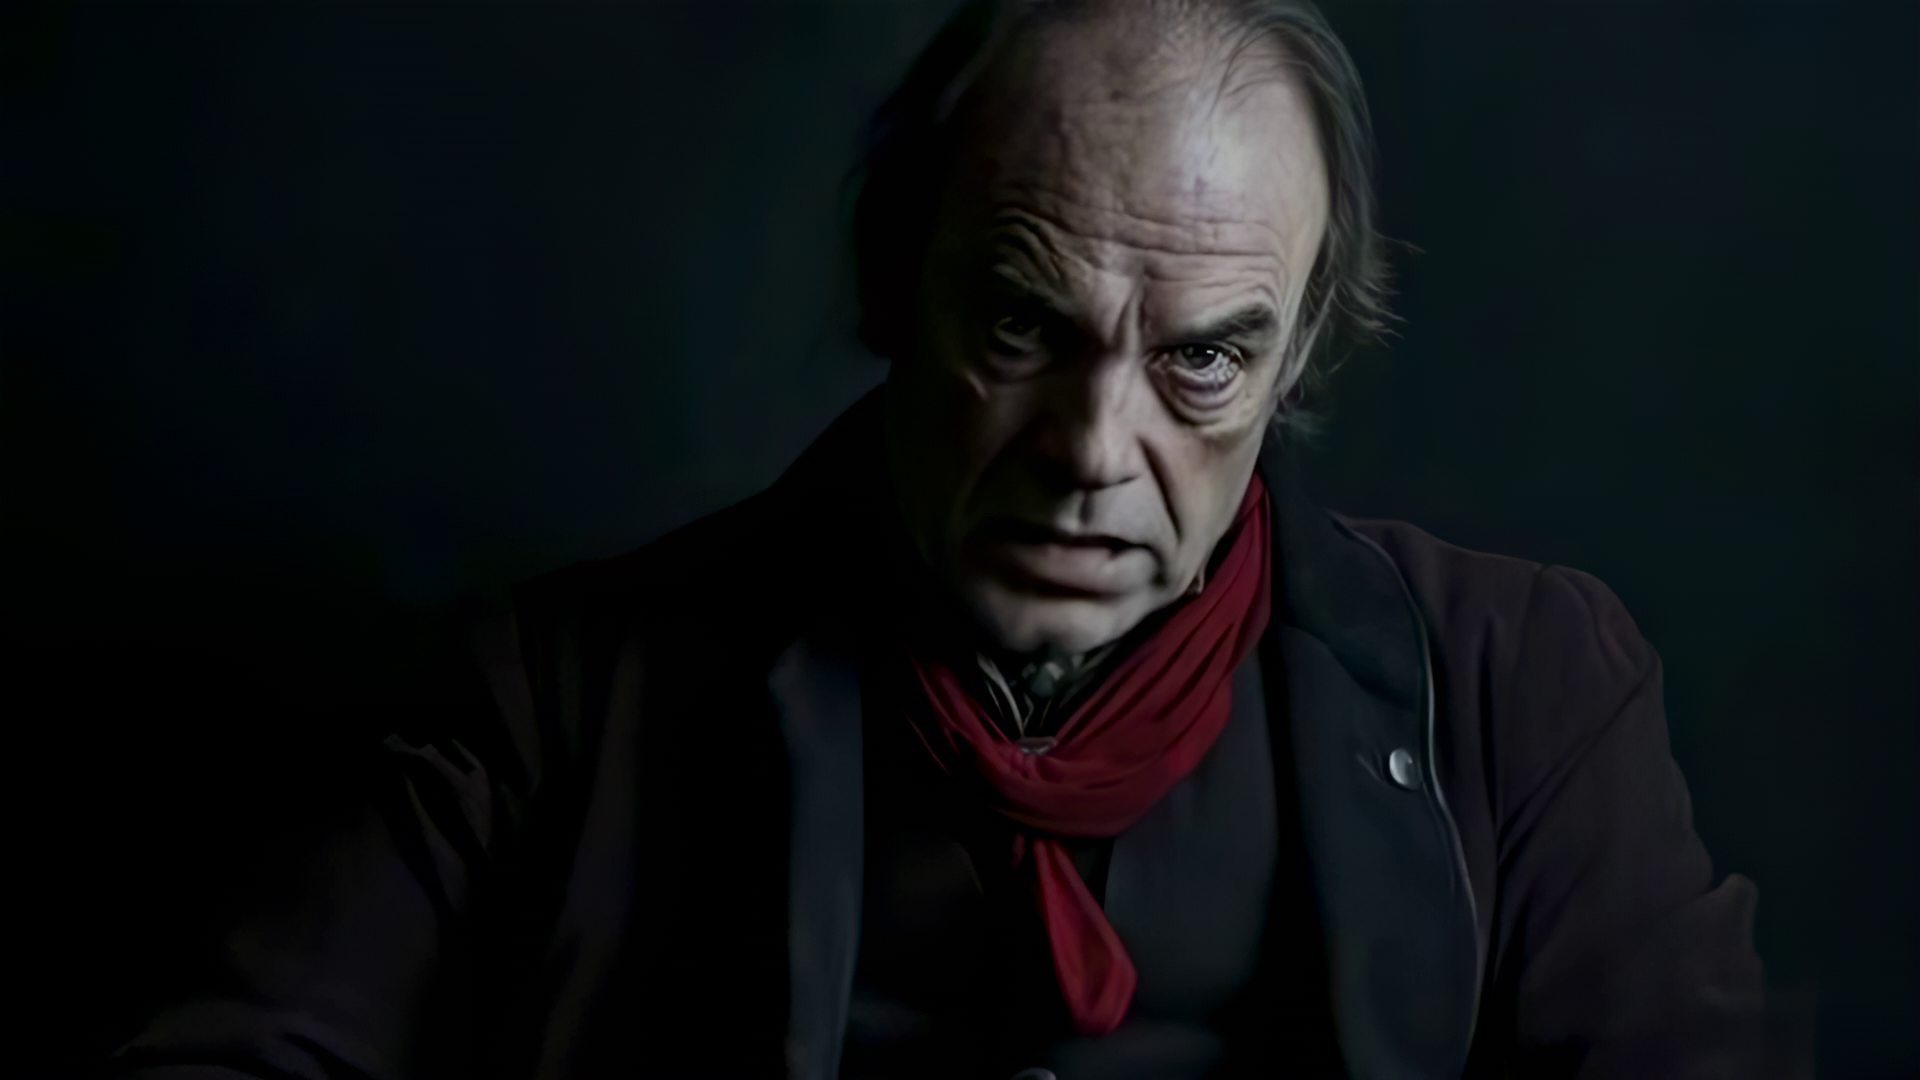
\includegraphics[width=2.5cm]{assets/ref_anger.png}} \par Reference image \par}
&
{\centering
\raisebox{-.5\height}{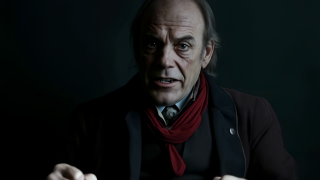
\includegraphics[width=2.5cm]{assets/Runway_anger.png}} \par A) Runway \par\vspace{0.3cm}
\raisebox{-.5\height}{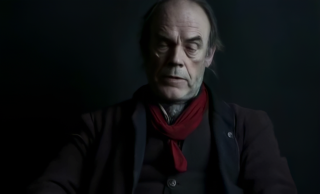
\includegraphics[width=2.5cm]{assets/Hunyuan_anger.png}} \par B) HunyuanVideo-Avatar \par}
&
\textbf{A) Runway (Rating: 5/10):} \textit{High visual quality and resolution, but the character has a relatively static face with a blank stare, lacking emotional micro-expressions. The eyes do not narrow and the brow remains un-furrowed despite the aggressive prompt.} \par\vspace{0.4cm}
\textbf{B) HunyuanVideo-Avatar (Rating: 2/10):} \textit{Severe face warping and distortion under high-intensity emotion. The jaw and mouth area show artifacting, and the teeth appear to float independently.}
&
\textbf{A) Runway (Rating: 6/10):} \textit{The anger feels superficial; the character's facial muscles do not contract realistically to match high-intensity rage. It looks like a neutral mask with an open mouth.} \par\vspace{0.4cm}
\textbf{B) HunyuanVideo-Avatar (Rating: 1/10):} \textit{The animation breaks suspension of disbelief due to temporal inconsistencies and facial stretching. The head moves in a jittery, disjointed motion.} \\
\midrule
{\centering
\raisebox{-.5\height}{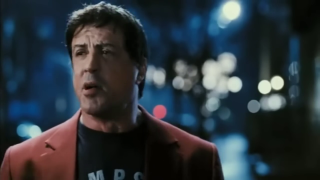
\includegraphics[width=2.5cm]{assets/actor_encouragement.png}} \par Encouragement scene \par\vspace{0.3cm}
\raisebox{-.5\height}{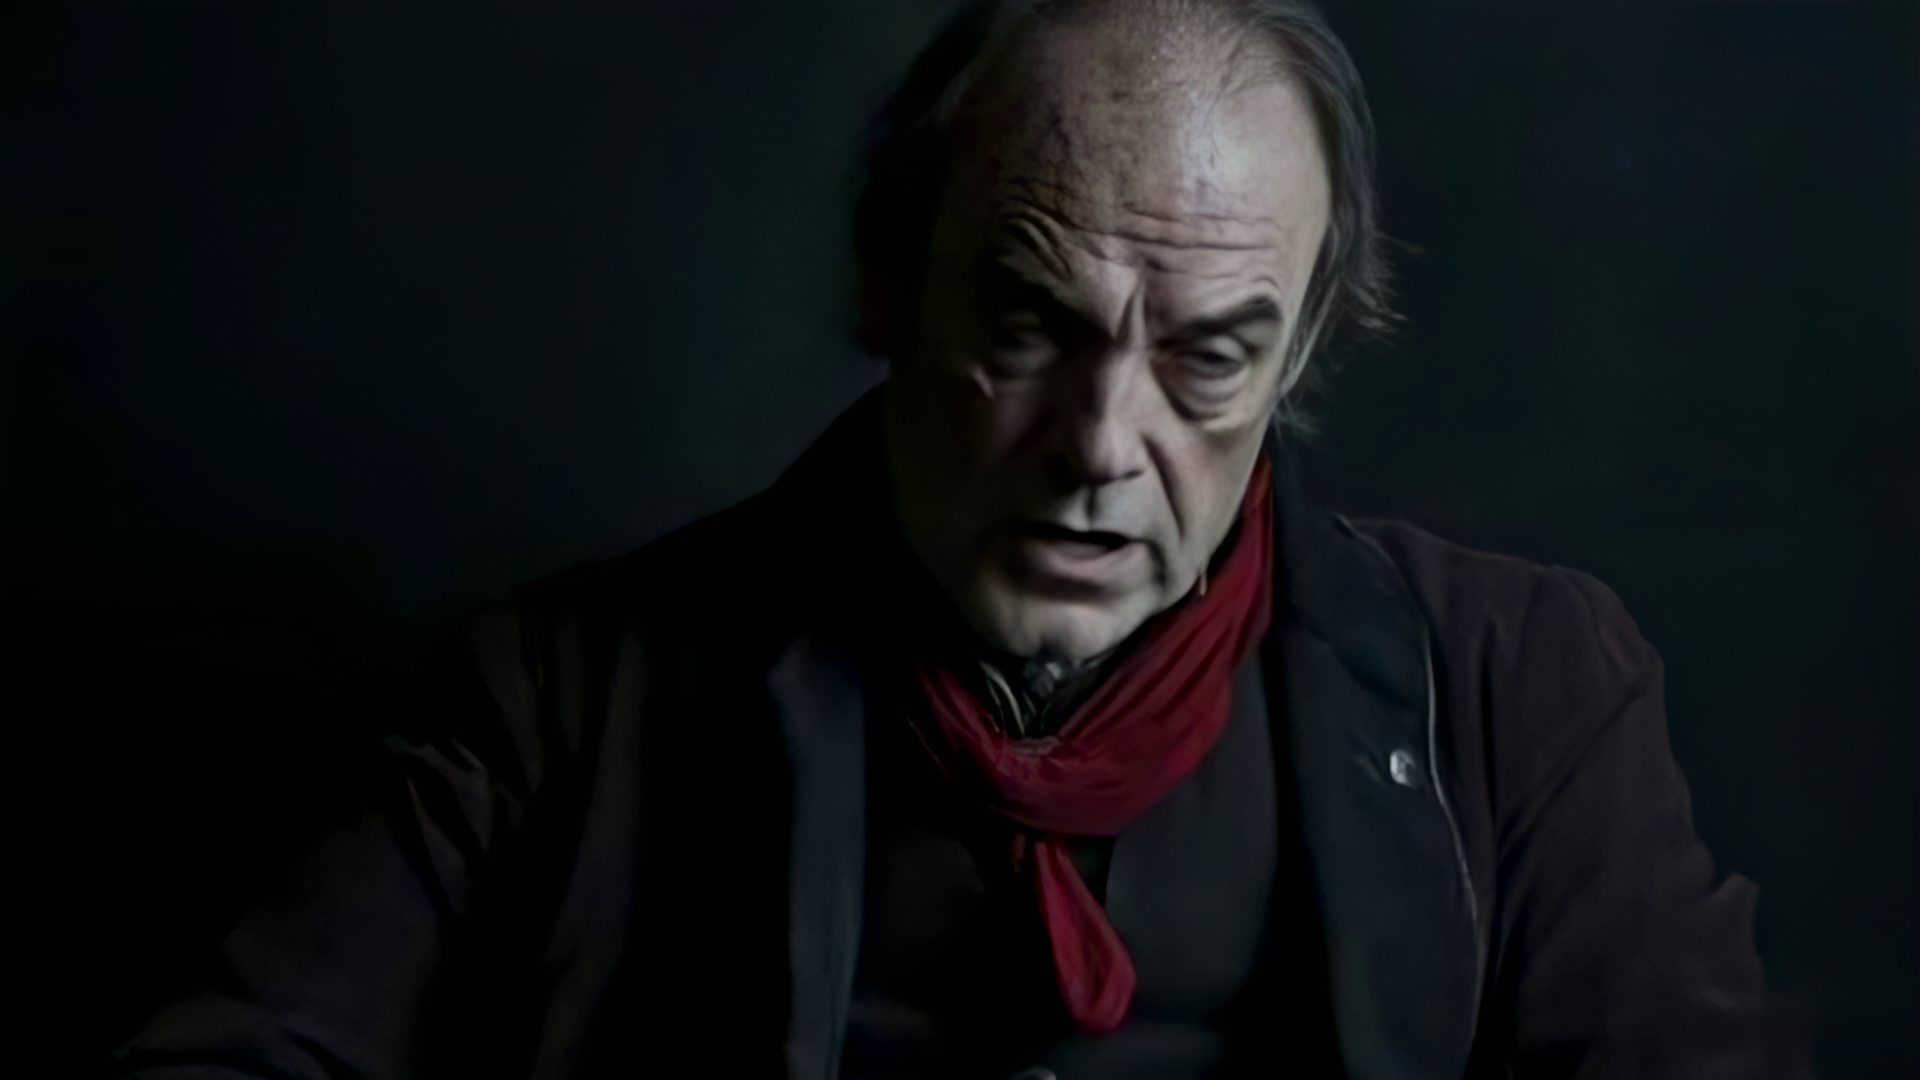
\includegraphics[width=2.5cm]{assets/ref_encouragement.png}} \par Reference image \par}
&
{\centering
\raisebox{-.5\height}{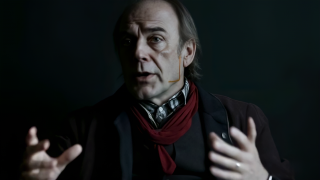
\includegraphics[width=2.5cm]{assets/Runway_encouragement.png}} \par A) Runway \par\vspace{0.3cm}
\raisebox{-.5\height}{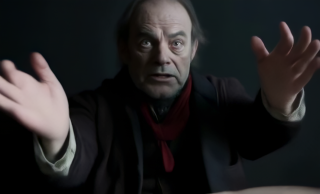
\includegraphics[width=2.5cm]{assets/Hunyuan_encouragement.png}} \par B) HunyuanVideo-Avatar \par}
&
\textbf{A) Runway (Rating: 5/10):} \textit{Steady head pose, but the eyes remain dead and unresponsive. The lips move to speak, but the rest of the face does not participate in the motivational delivery.} \par\vspace{0.4cm}
\textbf{B) HunyuanVideo-Avatar (Rating: 4/10):} \textit{Accurate lip-syncing but fails to connect vocal intensity with upper facial expressions, resulting in a disconnected and confusing performance.}
&
\textbf{A) Runway (Rating: 6/10):} \textit{The motivational expression is flat and robotic, lacking the nuance of a trained actor. The tone of voice suggests passion, but the face suggests indifference.} \par\vspace{0.4cm}
\textbf{B) HunyuanVideo-Avatar (Rating: 1/10):} \textit{Distortions occur in the cheek area during larger head movements, with skin textures appearing to slide over the underlying bone structure.} \\
\bottomrule
\end{tabular}%
}
\end{table*}

\begin{table*}[ht]
\centering
\caption{Expert Feedback on \emJoy and \emGratitude Expressions}
\label{tab:expert_feedback_joy_grat}
\makebox[\textwidth][c]{%
\begin{tabular}{p{2.8cm}p{2.8cm}>{\columncolor{gray!10}}p{5.0cm}>{\columncolor{gray!20}}p{5.0cm}}
\toprule
\textbf{Input} & \textbf{Output} & \textbf{P1} & \textbf{P2} \\
\midrule
{\centering
\raisebox{-.5\height}{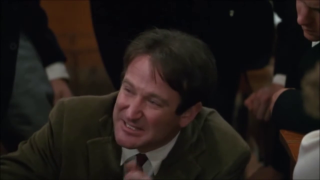
\includegraphics[width=2.5cm]{assets/actor_joy.png}} \par Joy scene \par\vspace{0.3cm}
\raisebox{-.5\height}{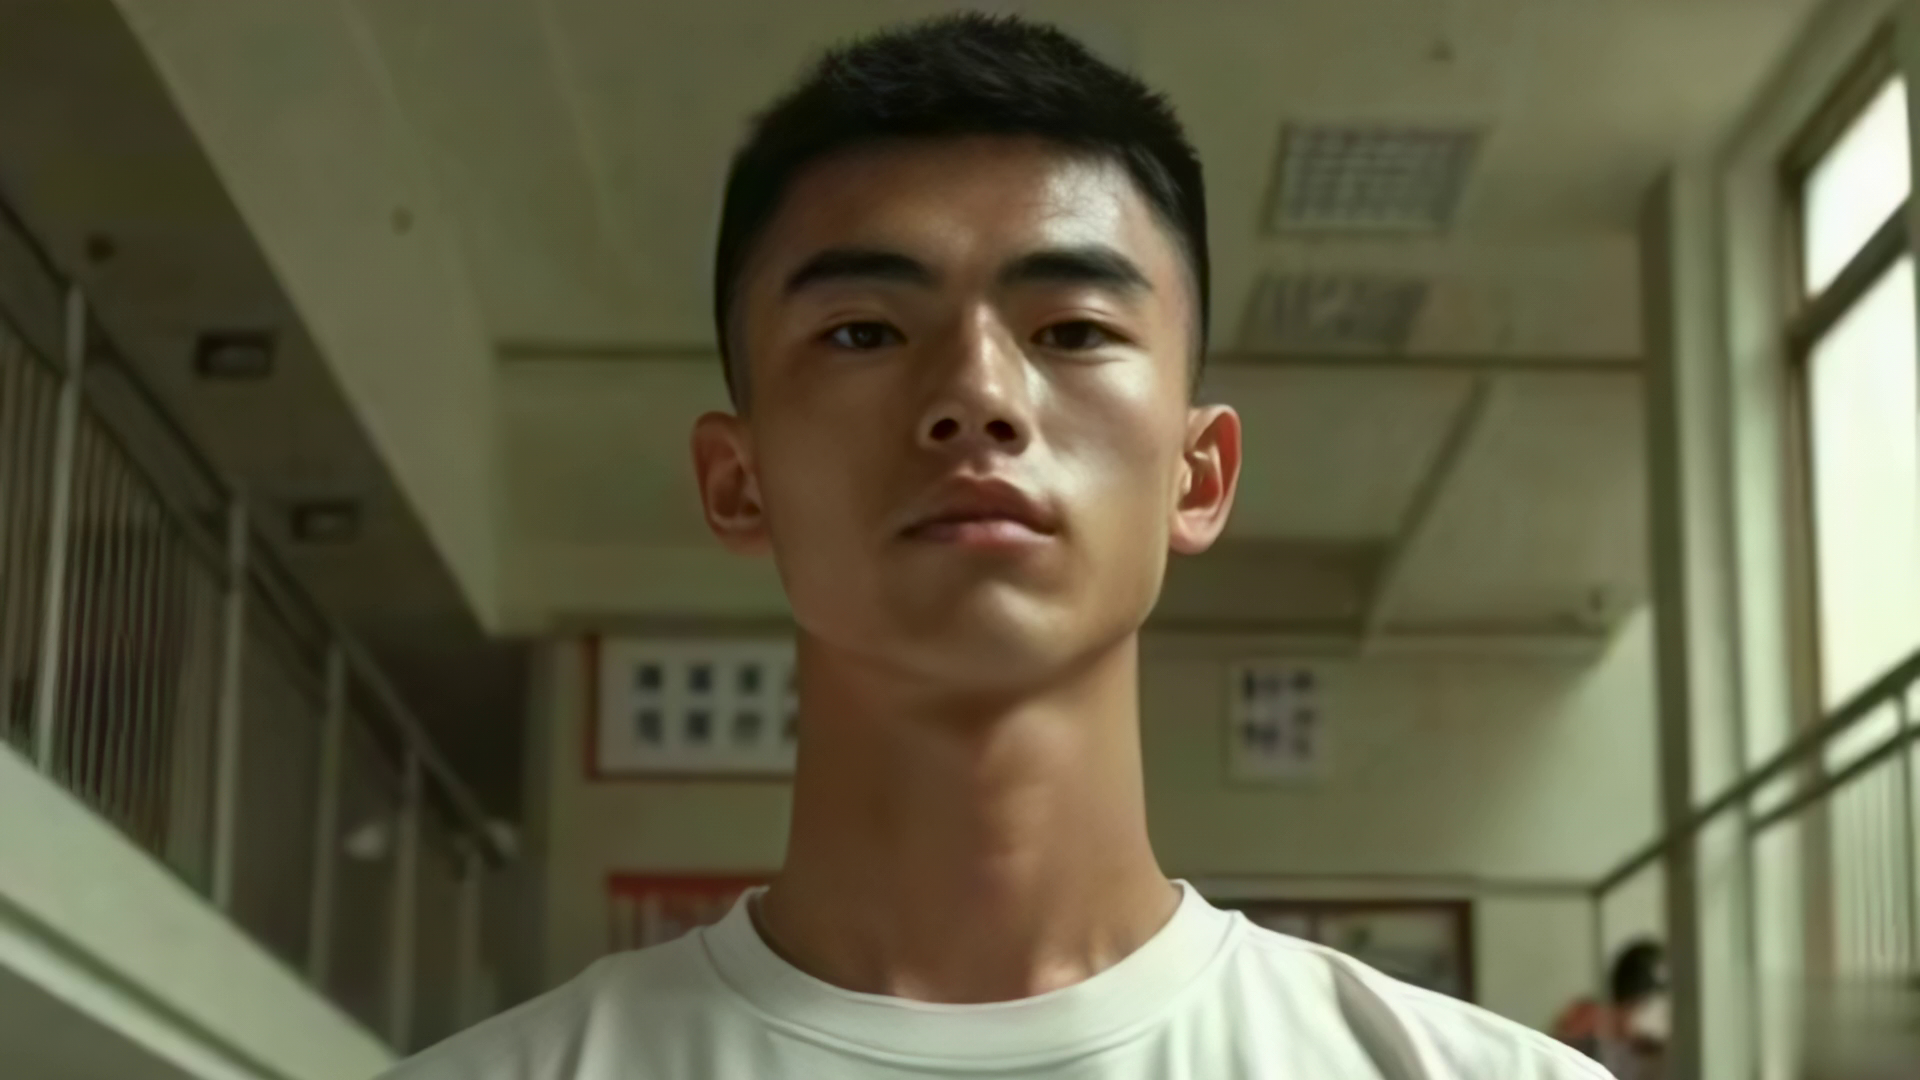
\includegraphics[width=2.5cm]{assets/ref_joy.png}} \par Reference image \par}
&
{\centering
\raisebox{-.5\height}{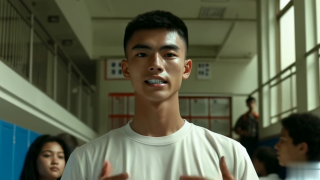
\includegraphics[width=2.5cm]{assets/Runway_joy.png}} \par A) Runway \par\vspace{0.3cm}
\raisebox{-.5\height}{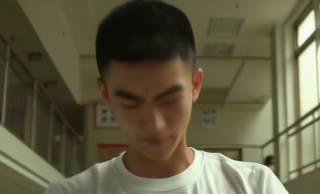
\includegraphics[width=2.5cm]{assets/Hunyuan_joy.png}} \par B) HunyuanVideo-Avatar \par}
&
\textbf{A) Runway (Rating: 5/10):} \textit{High aesthetic appeal, but the smile feels fake or ``plastic'', failing to engage the eyes (Duchenne smile deficit). The cheeks raise but the eyes do not crinkle.} \par\vspace{0.4cm}
\textbf{B) HunyuanVideo-Avatar (Rating: 4/10):} \textit{Struggles to keep facial structure stable while smiling, leading to melting or warping around the nose and mouth.}
&
\textbf{A) Runway (Rating: 2/10):} \textit{Looks like a stock photo animated; lacks the warm, natural transitions of genuine joy. The transitions between states are too linear and mechanical.} \par\vspace{0.4cm}
\textbf{B) HunyuanVideo-Avatar (Rating: 7/10):} \textit{Poor temporal coherence around the teeth and lips. The teeth seem to merge into a solid white block during the smile.} \\
\midrule
{\centering
\raisebox{-.5\height}{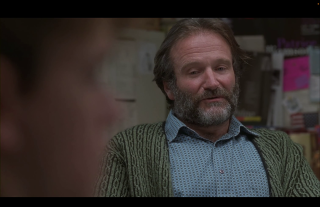
\includegraphics[width=2.5cm]{assets/actor_grateful.png}} \par Gratitude scene \par\vspace{0.3cm}
\raisebox{-.5\height}{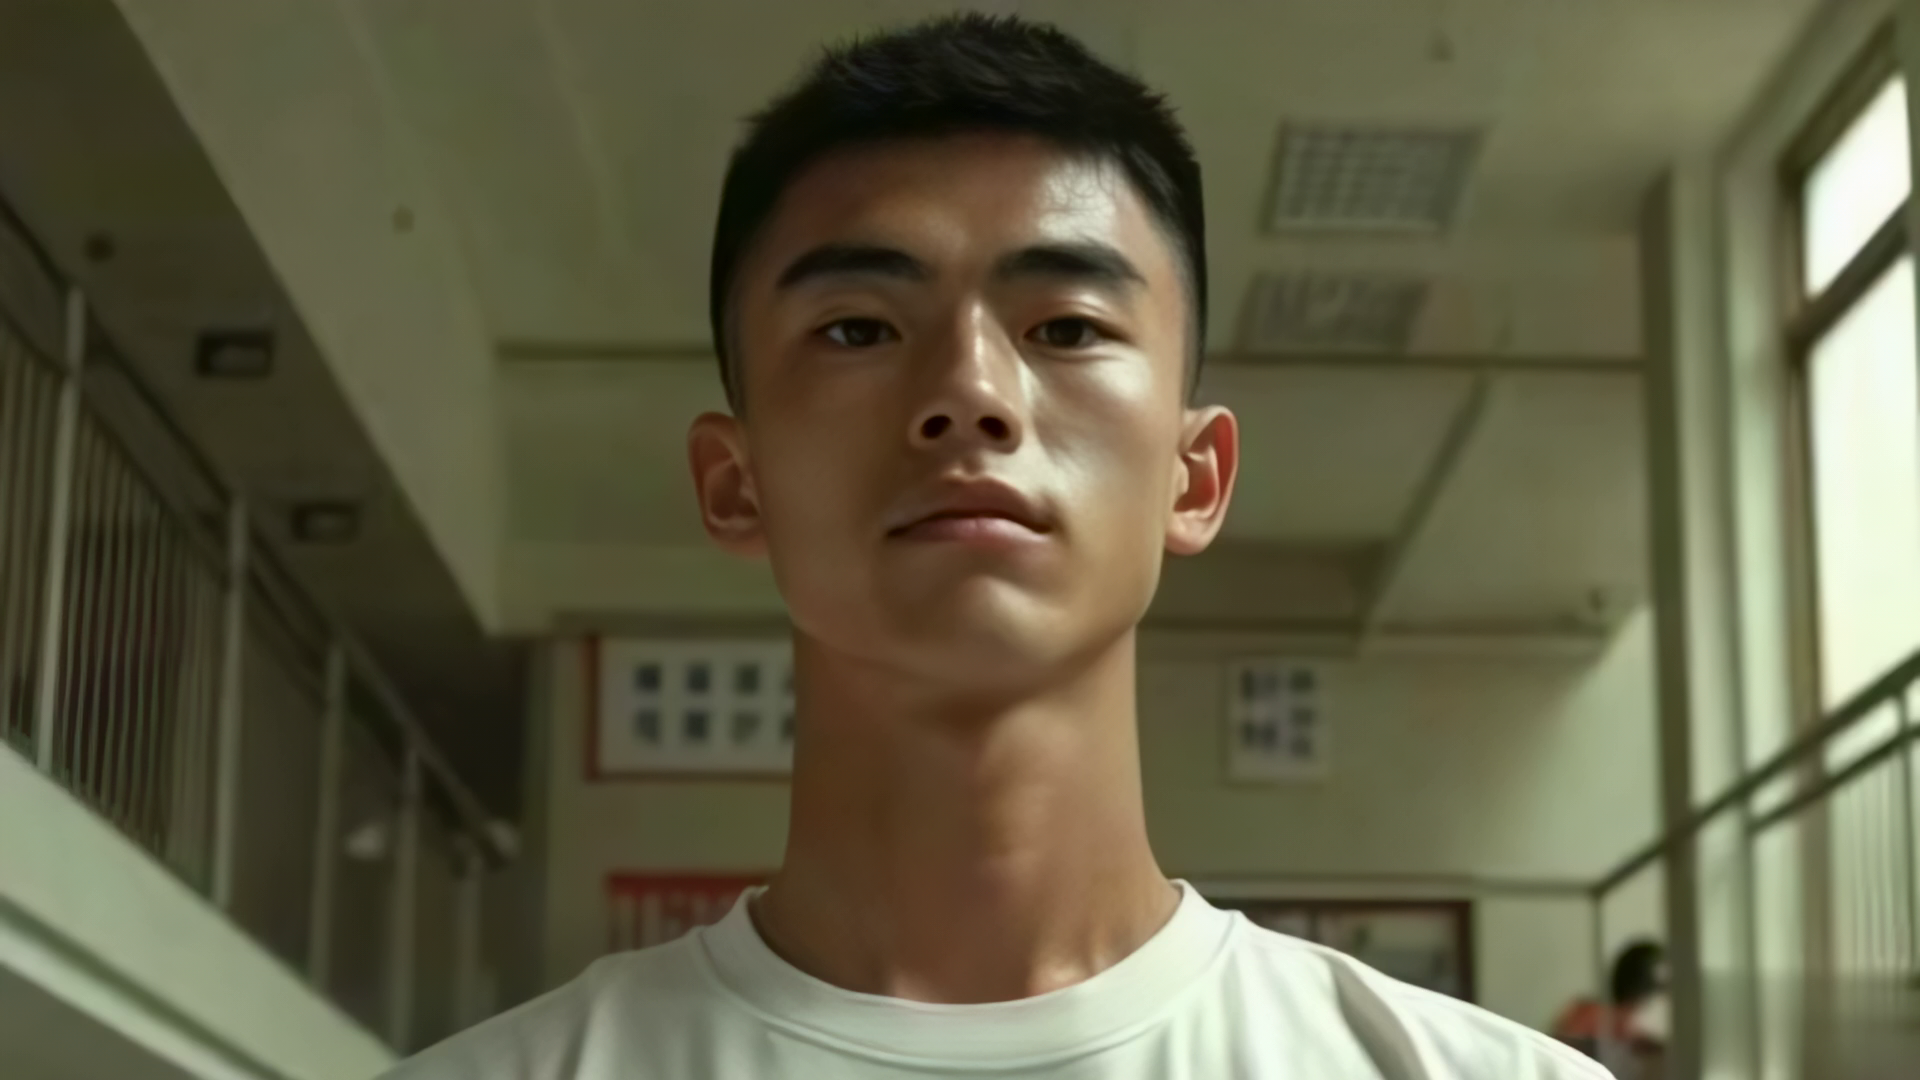
\includegraphics[width=2.5cm]{assets/ref_grateful.png}} \par Reference image \par}
&
{\centering
\raisebox{-.5\height}{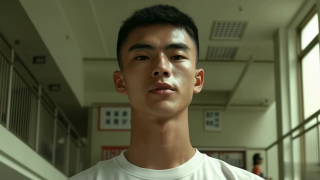
\includegraphics[width=2.5cm]{assets/Runway_grateful.png}} \par A) Runway \par\vspace{0.3cm}
\raisebox{-.5\height}{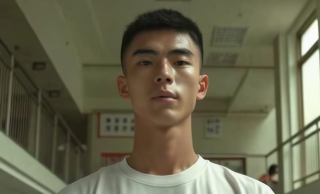
\includegraphics[width=2.5cm]{assets/Hunyuan_grateful.png}} \par B) HunyuanVideo-Avatar \par}
&
\textbf{A) Runway (Rating: 3/10):} \textit{The emotional tone is lost, resulting in a neutral or blank look rather than gratitude. The performance lacks the subtle facial softening that denotes appreciation.} \par\vspace{0.4cm}
\textbf{B) HunyuanVideo-Avatar (Rating: 4/10):} \textit{Cross-modal mismatch; voice is trembling and emotional, but the eyes are completely vacant, showing no recognition of the weight of the moment.}
&
\textbf{A) Runway (Rating: 6/10):} \textit{The character doesn't show the micro-expressions of vulnerability or emotion. It is too passive and fails to project any internal psychological state.} \par\vspace{0.4cm}
\textbf{B) HunyuanVideo-Avatar (Rating: 1/10):} \textit{The model cannot animate subtle eye movements (like welling up) to match the audio. The eye area remains static while the mouth shape changes.} \\
\bottomrule
\end{tabular}%
}
\end{table*}

\subsection{Somatic and Physiological Deficits in Generative Acting}\label{subsec:somatic_deficits}

A primary finding from our empirical focus group trials is the fundamental divergence between superficial visual photorealism and genuine somatic acting performance. While state-of-the-art Diffusion Transformers achieve convincing texture rendering, they fail across four interconnected somatic and physiological dimensions: anatomical muscle articulation, cross-modal affective alignment, autonomic physiological indicators, and grounded acting intentionality.

\begin{table*}[ht!]
\centering
\caption{Facial Action Coding System (FACS) Action Unit (AU) mapping and generative deficit analysis across evaluated emotions.}
\label{tab:facs_analysis}
\makebox[\textwidth][c]{%
\begin{tabular}{p{2.7cm}p{4.1cm}p{4.2cm}p{4.4cm}}
\toprule
\textbf{Emotion} & \textbf{Target Human AUs \& Muscles} & \textbf{Human Actor Somatic Execution} & \textbf{GenAI Generative Deficit} \\
\midrule
\emAnger & AU4 (Brow Lowerer, \textit{corrugator}), AU23 (Lip Tightener), AU24 (Lip Pressor) & Sustained contraction of corrugator supercilii, narrowing palpebral fissure, tensed lips under vocal strain & Brow remains flat and unknitted; lips open mechanically; vacant ocular stare (``slack mask'') \\
\addlinespace
\emEncouragement & AU1 (Inner Brow Raiser), AU2 (Outer Brow Raiser), AU14 (Dimpler, \textit{buccinator}) & Attentive ocular fixation, empathetic frontalis engagement, affirmative head-nodding cadence & Static upper facial third; head drifts unnaturally; vocal passion decoupled from facial warmth \\
\addlinespace
\emJoy & AU6 (Cheek Raiser, \textit{orbicularis oculi}), AU12 (Lip Corner Puller, \textit{zygomaticus}) & True Duchenne smile: involuntary contraction of pars orbitalis crinkling periocular tissue & Isolated AU12 execution; complete absence of AU6 contraction; rigid, plastic grimace \\
\addlinespace
\emGratitude & AU1 (Inner Brow Raiser), AU15 (Lip Corner Depressor), AU17 (Chin Raiser) & Vulnerable somatic softening, trembling lower lip, tear meniscus accumulation, cathartic release & Flat, inert eye area; mouth moves without psychological depth; emotional trembling absent \\
\bottomrule
\end{tabular}%
}
\end{table*}

\textbf{Facial Action Coding System (FACS) Breakdown.} Grounded in Ekman and Friesen's Facial Action Coding System~\cite{ekman1978facial}, human emotional expression requires precisely coordinated co-activations of discrete facial muscle groups (Table~\ref{tab:facs_analysis}). In our empirical trials, generative models consistently failed to reproduce these anatomical synergies:
\begin{itemize}
    \item \textit{\emAnger:} In Jack Nicholson's courtroom monologue, authentic fury requires intense recruitment of AU4 (Brow Lowerer / \textit{corrugator supercilii}), alongside AU23 (Lip Tightener) and AU24 (Lip Pressor / \textit{orbicularis oris}). Neither Runway nor HunyuanVideo-Avatar successfully engaged AU4; the brow remained smooth and un-furrowed despite acoustic shouting. HunyuanVideo-Avatar attempted to depict anger through severe geometric stretching of the jaw rather than localized muscular contraction, causing teeth to float independently.
    \item \textit{\emJoy:} In Robin Williams' classroom sequence, human joyousness manifests through a authentic Duchenne smile requiring simultaneous activation of AU12 (Lip Corner Puller / \textit{zygomaticus major}) and involuntary AU6 (Cheek Raiser / \textit{orbicularis oculi, pars orbitalis}). Both models exhibited an acute Duchenne smile deficit: the mouth corners were pulled back (AU12), but the orbicularis oculi (AU6) remained flaccid. The absence of lower eyelid elevation and lateral canthus wrinkles (``crow's feet'') produced an insincere, synthetic grimace that both \Pone and \Ptwo described as ``plastic'' and resembling an ``animated stock photo.''
    \item \textit{\emGratitude:} In the counseling scene from \textit{Good Will Hunting}, cathartic emotional release depends on subtle frontalis medialis engagement (AU1: Inner Brow Raiser) and depressor anguli oris (AU15: Lip Corner Depressor), creating a somatic softening of the upper face. Generative avatars maintained a deadpan ocular expression, completely divorcing the visual face from the vulnerable auditory delivery.
    \item \textit{\emEncouragement:} Sylvester Stallone's motivational speech relies on synchronized AU1/AU2 activation paired with concentrated, unwavering eye contact. Generative models rendered an unblinking, robotic stare where the lower face articulated speech while the upper face displayed complete indifference.
\end{itemize}

\textbf{Cross-Modal Audio-Visual Disconnect and the Viseme Illusion.} A major architectural limitation uncovered in our trials is the cross-modal decoupling between acoustic speech conditioning and upper-facial kinesics. Audio-driven diffusion frameworks (e.g., HunyuanVideo-Avatar) process speech audio through self-supervised encoders (such as Wav2Vec 2.0~\cite{baevski2020wav2vec} or HuBERT) to extract frame-level acoustic embeddings, conditioning the Diffusion Transformer via cross-attention layers. However, acoustic speech representations primarily correlate with vocal tract articulators---namely the jaw, lips, and tongue (visemes corresponding to phonetic transitions such as bilabials or fricatives). Standard avatar training objectives emphasize lip synchronization accuracy (e.g., SyncNet discrimination or lower-face landmark loss). Consequently, the gradient update strongly drives mouth articulation, but provides zero supervisory signal or causal conditioning for the upper facial third. Because the speech waveform does not deterministically prescribe periocular or corrugator muscle activation, cross-attention leaves the upper face unconstrained. In the absence of an explicit affective conditioning pathway, the diffusion sampling process defaults to the empirical mode of the training prior---rendering an unexpressive, neutral upper face (``dead eyes'') even when the vocal track conveys sobbing, trembling grief, or rage.

\textbf{Autonomic and Physiological Deficits.} Authentic acting performance is embodied in involuntary physiological responses regulated by the sympathetic and parasympathetic nervous systems. Human spectators sub-perceptually register these autonomic signals to gauge emotional authenticity:
\begin{enumerate}
    \item \textit{Pupillary Dynamics:} Autonomic arousal in rage and joy triggers pupil dilation (mydriasis), whereas emotional calming induces constriction (miosis). Both generative models render static, invariant pupils across all emotional transitions.
    \item \textit{Vascular Perfusion and Blushing:} Psychological stress and emotional arousal modulate cutaneous microvascular blood flow, causing flushing across the zygomatic arches, nose, and ears under anger, or paleness under shock. Latent diffusion models synthesize static skin albedo without hemodynamic modeling.
    \item \textit{Neuromuscular Micro-Tremors:} Intense suppressed emotion (such as gratitude or grief) induces involuntary high-frequency micro-tremors in the mentalis muscle (quivering chin) and lip margins. Generative avatars execute smoothed, linearly interpolated motion trajectories that eliminate natural somatic tremors.
    \item \textit{Tear Meniscus and Ocular Hydration:} Emotional catharsis stimulates lacrimal gland excretion, accumulating a reflective tear meniscus along the lower eyelid margin and altering corneal specular highlights. Generative models produce dry, glassy eyes that remain unchanged regardless of emotional intensity.
    \item \textit{Respiratory Cadence:} Human speech is physically grounded in respiratory mechanics---chest expansion, clavicular rise, nostril flaring, and audible catch-breaths. Generative models treat speech audio as an isolated acoustic stream, synthesizing an animated head floating without somatosensory respiratory anchoring.
\end{enumerate}

\textbf{Acting Pedagogy: Somatic Craft vs. Statistical Likelihood Sampling.} The profound expressive gap between human performers and generative avatars is fundamentally rooted in divergent philosophies of performance. In theatrical and cinematic acting theory:
\begin{itemize}
    \item Konstantin Stanislavski's \textit{System}~\cite{stanislavski1936actor} established the principle of ``psycho-physical action'': emotion is never an external cosmetic pose or superficial facial mimicry; rather, it is the emergent somatic consequence of an actor pursuing an ``inner objective'' within the ``magic if.'' Physical actions trigger authentic feelings, which in turn manifest as involuntary micro-kinesics across the human anatomy.
    \item Lee Strasberg's \textit{Method}~\cite{strasberg1987dream} expanded on affective memory and sensory recall, wherein an actor's vivid somatic re-experience of past sensory stimuli activates autonomic nervous system pathways that cannot be simulated through conscious mechanical effort alone.
    \item Sanford Meisner's technique~\cite{meisner1987acting} posits that truthful acting stems from the ``reality of doing'' and instinctive, moment-to-moment listening and adaptation to an interlocutor in real time.
\end{itemize}
In stark contrast, generative diffusion architectures operate under a purely mathematical formulation: maximizing conditional data likelihood or traversing deterministic Flow Matching trajectories~\cite{lipman2022flow} in latent space. Conditioned solely on text tokens or speech spectrogram frames, the model treats performance as the sampling of superficial texture correlations. Because latent diffusion operates in the total absence of an intentional consciousness, an inner objective, autonomic physiology, or relational awareness of an interlocutor, it produces only superficial pantomime. It delivers the outward illusion of human appearance without the internal somatic reality of human performance.

\subsection{Quality Dimensions}\label{sec5:technical}

Our evaluation demonstrates a fundamental divergence between surface visual fidelity and deep emotional performance synthesis across generative architectures. Synthesizing feedback from our focus group across the test scenes, we structure our analysis around four core Quality Dimensions:

\textbf{Aesthetic Quality.} We consider Aesthetic Quality to measure overall visual fidelity, resolution, and surface skin texture rendering. Proprietary models (Runway) achieve exceptional visual polish, whereas open-source models (HunyuanVideo-Avatar) show minor texture artifacts; however, high aesthetic quality does not correlate with emotional expressiveness.

\textbf{Expression Realism.} We consider Expression Realism to evaluate anatomical accuracy and action unit articulation. While HunyuanVideo-Avatar displays more dynamic facial muscle engagement than Runway during high-intensity monologues (e.g., Jack Nicholson's \emAnger), both pipelines lack biophysical skeletal constraints, producing unnatural jaw float and lip drift.

\textbf{Emotional Intensity.} We consider Emotional Intensity to assess psychological depth and cross-modal alignment between audio and facial kinesics. Both models exhibit severe emotional flattening (``dead eyes'') and Duchenne smile deficits during genuine joy (Robin Williams in \textit{Dead Poets Society}) and cathartic vulnerability (Robin Williams and Matt Damon in \textit{Good Will Hunting}), where trembling voice audio fails to animate upper facial micro-expressions.

\textbf{Temporal Coherence.} We consider Temporal Coherence to track identity stability and motion continuity over time. Commercial pipelines preserve static facial identity effectively, whereas open-source models suffer from face warping and skin sliding under rapid head movements (e.g., Sylvester Stallone in \textit{Rocky Balboa}).

Ultimately, because diffusion transformers process video as sequences of unconstrained spatial-temporal patches rather than biomechanically bounded anatomical structures, they fail to replicate the holistic physical process---such as involuntary micro-expressions and autonomic kinesics---that defines authentic human acting.


\section{Societal Impact}\label{sec5:societal}

The deployment of generative video models in media production cannot be considered solely from a technical perspective. The adoption of AI avatars by organizations without adequate compliance standards introduces severe legal, financial, and reputational risks. The ScotRail 2025 case study~\cite{pavis2025ai, signapselinkedin} illustrates this vulnerability: an AI-generated voice announcement system, built from a digital clone of actor Gayanne Potter, was deployed without her explicit knowledge or consent, leading to public controversy and potential litigation. As generative tools transition from experimental prototypes to commercial production pipelines, evaluating technical performance fidelity must be paired with an examination of broader societal, ethical, and legal ramifications. 


\subsection{Ethical Dimensions}

To systematically address these complex challenges, we propose examining four core Ethical Dimensions below.

\textbf{Model Auditability and Data Opacity.} Bridging our technical evaluation with broader societal concerns, the trade-off between model auditability and performance fidelity introduces significant governance challenges. Currently available open-source architectures (such as HunyuanVideo-Avatar) are fully auditable and inspectable, allowing researchers to examine code structures and internal representations; however, as demonstrated in our emotional fidelity evaluation, these models currently yield inferior expressive results, exhibiting severe facial warping, tooth float, and structural instability. Conversely, commercial proprietary models (such as Runway Gen-3) achieve higher aesthetic polish, but their underlying training datasets, data provenance, and scraping sources remain completely opaque and un-auditable. This lack of transparency hides potential copyright infringements, consent violations, and unauthorized likeness ingestion, creating substantial legal and ethical risks for creative industries and archival preservation.

\textbf{Ethical Archiving.} The limitations in emotional fidelity have immediate implications for the responsible deployment of GenAI in creative fields~\cite{braid2024responsible}. Rather than positioning generative models as autonomous replacements for human performers, they should be treated as collaborative tools, primarily suitable for pre-visualization, storyboarding, or low-stakes background elements. In digital archiving, the creation of synthetic performances of deceased actors from historical audio or video recordings raises serious ethical concerns regarding authenticity and consent. Archivists and cultural curators must establish boundaries between authentic historical records and generative reconstructions to maintain historical and institutional integrity.

\textbf{Labor Safeguards.} The vulnerability of creative workers was brought to international prominence during the 118-day 2023 SAG-AFTRA strike, which centered on establishing contractual protections against unauthorized generative replicas. The resulting 2023 TV/Theatrical Agreement~\cite{sagaftra2023summary} codified specific definitions for "digital replicas" (both employment-based and independent), requiring explicit, conspicuous consent and bargaining-scale compensation whenever an actor's digital counterpart is synthesized. Crucially, as noted in the policy report by Pavis and Lees~\cite{pavis2025ai, signapselinkedin}, the uncontrolled adoption of digital cloning tools risks displacing creative and technical professionals—including actors, voice artists, translators, and customer support representatives. Moreover, the deployment of AI avatars in sensitive sectors like education, healthcare, or memorialisation introduces significant risks of emotional dependency and reduced human interaction, which must be carefully governed. The reliance on contracts to govern digital avatars in the absence of robust statutory rights often reinforces power asymmetries between workers and technology developers. The Pavis and Lees policy briefing~\cite{pavis2025ai, signapselinkedin} reports the widespread inclusion of perpetual "buy-out" clauses in employment and freelance contracts. These clauses pressure performers to assign their likeness data and digital cloning rights indefinitely as a condition of employment, stripping them of long-term consent, creative control, and fair compensation. To counter this, statutory protections are needed to render perpetual transfers of digital likeness unenforceable, ensuring that consent is always specific, informed, and revocable. Government policy must support collective bargaining and roundtables involving unions (such as SAG-AFTRA, Equity, the Trades Union Congress - TUC, and the University and College Union - UCU) to establish standard fair terms. Reference resources like Equity's AI toolkit and the European Union of the Deaf's contract framework offer valuable templates for structuring these protections.

\textbf{Corporate Compliance.} The rapid expansion of digital cloning exposes critical regulatory gaps in current legal frameworks governing digital likeness. As detailed by Pavis and Lees~\cite{pavis2025ai, signapselinkedin}, statutory protections such as the UK Copyright, Designs and Patents Act 1988 (CDPA) cover recorded performances but omit digital clones, leaving performers vulnerable to unauthorized replication across fragmented regulations. To mitigate compliance and reputational liabilities, organizations must establish rigorous procurement protocols mandating due diligence on data provenance, model ownership, and licensing validity. Furthermore, regulatory bodies (DSIT, IPO, and ICO) should establish unified statutory likeness rights and risk-management frameworks to protect performers' image, voice, and identity rights.

\subsection{International Regulatory Frameworks and Authorship}\label{subsec:regulatory}

Beyond collective bargaining and corporate procurement protocols, the governance of synthetic avatars operates across divergent international regulatory regimes. Addressing RQ2 requires examining how statutory mandates in the European Union, copyright doctrine in the United States, and emerging policies in the United Kingdom approach synthetic media, emotion recognition, and digital authorship.

\textbf{The EU AI Act: High-Risk Biometrics and Mandatory Transparency.} The European Union's Artificial Intelligence Act (Regulation EU 2024/1689)~\cite{euaiact2024} represents the first comprehensive horizontal statutory regime for AI, establishing stringent obligations for synthetic media and biometric processing. Under Article 50 of the Act, providers and deployers of AI systems that generate or manipulate audio-visual content constituting deepfakes face mandatory transparency obligations: synthetic outputs must be explicitly disclosed and watermarked in a machine-readable format, with only narrow exceptions for artistic parody or authorized investigative uses. Crucially, the EU AI Act also adopts a precautionary stance toward affective computing, categorizing emotion recognition systems in workplace and educational environments as high-risk or prohibited due to their scientific unreliability and risk of psychological manipulation. As our technical evaluation demonstrates, generative video models map facial kinematics purely as statistical correlations rather than authentic somatic affective states; deploying synthetic avatars in public or interactive settings without verified provenance risks violating the EU's biometric governance mandates.

\textbf{United States Copyright Office: Non-Human Authorship Doctrine.} In contrast to the European regulatory focus on fundamental rights and risk classification, the United States has primarily addressed generative media through the lens of intellectual property and copyrightability. The US Copyright Office (USCO) 2023 Policy Guidance on Works Containing Material Generated by Artificial Intelligence~\cite{usco2023guidance}—anchored by judicial rulings in \textit{Thaler v. Perlmutter} and the registration determination in \textit{Zarya of the Dawn}—mandates that copyright protection strictly requires human authorship. Audio-visual content generated solely through text prompts or statistical diffusion processes lacks human creative control and cannot be copyrighted per se; copyright can only attach to human-authored arrangement, selection, or subsequent physical editing. This doctrine introduces a major economic paradox for the film industry: while studios may deploy GenAI avatars to reduce production expenses, synthetic characters and autonomous performances remain in the public domain or lack enforceable proprietary copyright, severely undermining the commercial value of purely synthetic intellectual property. Concurrently, because federal copyright does not recognize digital likeness rights, performers in the US must navigate an inconsistent patchwork of state-level Right of Publicity statutes (or emerging federal proposals like the NO FAKES Act) to protect their somatic identity against unauthorized cloning.

\textbf{Comparative Governance Synthesis.} Table~\ref{tab:regulatory_frameworks} summarizes the key regulatory approaches across the European Union, United States, and United Kingdom. While the UK currently relies on existing intellectual property statutes (CDPA 1988) with acknowledged gaps in synthetic likeness governance~\cite{pavis2025ai}, the EU prioritizes mandatory watermarking and biometric safeguards under the EU AI Act~\cite{euaiact2024}, and the US couples a strict human-authorship copyright doctrine~\cite{usco2023guidance} with union-negotiated contractual standards~\cite{sagaftra2023summary}. For creative industries and archival institutions, responsible adoption requires harmonizing technical auditability (RQ2) with these divergent international compliance mandates.

\begin{table}[ht!]
\caption{Comparison of International Regulatory Frameworks Governing Generative Avatars and Synthetic Media.}\label{tab:regulatory_frameworks}
\begin{tabular}{p{2.0cm} | @{\foo} p{2.6cm} | @{\foo} p{2.6cm} | @{\foo} p{3.3cm}}
\toprule
\textbf{Jurisdiction} & \textbf{Primary Instrument} & \textbf{Core Mechanism} & \textbf{Impact on AI Avatars} \\
\midrule
European Union & EU AI Act (2024/1689)~\cite{euaiact2024} & Article 50 Transparency; Risk Tiers & Mandatory machine-readable watermarking; curbs on emotion recognition systems \\
United States & USCO Guidance (2023)~\cite{usco2023guidance} & Human Authorship Doctrine & Pure GenAI avatar outputs uncopyrightable; reliance on state publicity rights \\
United States (Labor) & SAG-AFTRA Agreement (2023)~\cite{sagaftra2023summary} & Collective Bargaining & Mandatory consent and scale pay for digital replicas; bans on unconsented scans \\
United Kingdom & CDPA 1988 \& Pavis-Lees~\cite{pavis2025ai} & Existing IP / Sectoral Regulators & Statutory gaps in digital likeness protection; vulnerability to perpetual buy-out clauses \\
\bottomrule
\end{tabular}
\end{table}

\section{Final Remarks}\label{sec6}
In addressing our central research questions, a key contribution of this work is proposing both Quality Dimensions and Ethical Dimensions. First, in response to RQ1 regarding emotional fidelity, we propose four core Quality Dimensions (Aesthetic Quality, Expression Realism, Emotional Intensity, and Temporal Coherence). Our findings reveal that while current models achieve good aesthetic standards, they remain fundamentally limited in expression realism and emotional intensity, lacking the physical coordination, anatomical constraints, and expressive intentionality of a trained actor. Second, in response to RQ2 regarding model inspectability, we propose Ethical Dimensions surrounding model auditability, dataset provenance, and digital likeness rights, contrasting international regulatory regimes including the EU AI Act (mandatory watermarking and biometric limits) and US Copyright Office doctrines (human authorship constraints). We highlight that while open-source models (HunyuanVideo-Avatar) are fully auditable, they currently yield inferior expressive quality, whereas proprietary models (Runway) achieve higher surface aesthetics at the cost of complete dataset opacity.

To advance the responsible integration of GenAI in cinematic production and archival preservation, future research must shift focus from surface visual polish to emotion-conditioned internal representations (i.e., latent spaces) grounded in human kinesics and anatomical priors. We advocate for developing auditable, open-source architectures that integrate biomechanical constraints and consent-driven likeness licensing, fostering an ethical, transparent partnership between generative technology and human performance art.

\phantomsection
\bmhead{Acknowledgments}
This work was supported by [Anonymized Funding]. We thank the participants from the [Anonymized Department].

\bibliography{references}

\end{document}
